%==============================================================================
% BAB IV: METODE PENELITIAN
% [Catatan]: Rincian subbab dapat disesuaikan dengan output pekerjaan PKL Anda.
%==============================================================================
\chapter{Metode Penelitian}

\pet{Pada bagian ini dijelaskan mengenai pelaksanaan PKL meliputi deskripsi persoalan, alur proses penyelesaian, gambaran umum, dan metodologi pengembangan dari perangkat lunak, keras, sistem, dan prototype yang dikembangkan atau dibangun. Adapun rincian dari substansi pada Bab IV adalah sebagai subbab berikut, tetapi subbab dapat disesuaikan kembali dengan output yang anda kerjakan pada tempat kerja praktek anda.}

\pet{Caption tabel dan gambar ditulis dengan format <bab>.<urutan tabel/gambar>. Caption tabel berada di atas tabel, sedangkan caption gambar berada di bawah gambar.}

\begin{table}[H]
  \centering
  \caption{Contoh \textit{caption} tabel}
  \spasisatu
  \setlength{\arrayrulewidth}{1pt}
  \begin{tabular}{|p{4.35cm}|p{4.35cm}|p{4.35cm}|}
    \hline
    \rule{0pt}{14pt} & & \\
    \hline
    \rule{0pt}{14pt} & & \\
    \hline
    \rule{0pt}{14pt} & & \\
    \hline
  \end{tabular}
\end{table}

\begin{figure}[H]
  \centering
  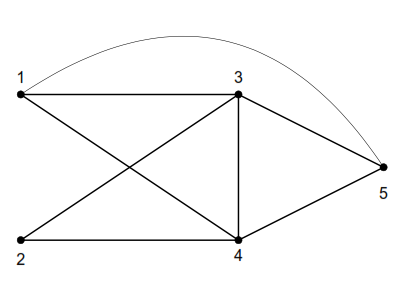
\includegraphics[width=5.95cm,height=4.47cm]{figure/contoh-gambar.png}
  \caption{Contoh \textit{caption} gambar}
\end{figure}

\section{Analisis Permasalahan}
\pet{Tuliskan analisis dari persoalan yang harus diselesaikan dalam kerja praktek, termasuk usulan solusi untuk persoalan tersebut. Sesuaikan dengan latar belakang persoalan, deskripsi persoalan, batasan yang harus diselesaikan dalam PKL, teknologi terkait yang mendukung solusi dari persoalan, dan hal lain yang terkait dengan persoalan PKL.}

\section{Alur Penyelesaian}
\pet{Tuliskan alur penyelesaian PKL anda dengan detail, dari mulai observasi, identifikasi masalah, perumusan masalah, pemilihan metode, implementasi, pengujian, dan penarikan kesimpulan. Supaya lebih tergambar dengan jelas, bisa dengan menggunakan \textit{flowchart}.}

\section{Gambaran Umum Sistem/Aplikasi/Prototype}
\pet{Gambarkanlah secara umum terkait arsitektur sistem/aplikasi/prototype yang anda kembangkan. Dapat menggunakan diagram atau gambar sebagai pembantu.}

\section{Alat dan Bahan}
\pet{Uraikan spesifikasi dari alat dan bahan yang digunakan untuk mendukung pengembangan sistem atau prototype.}

\subsection{Alat}
\pet{Alat yang digunakan untuk melakukan pengembangan sistem atau prototype, dapat berupa komputer, PC, Arduino, raspberry, dsb.}

\begin{enumerate}
  \item Notebook, dengan spesifikasi…
  \item Smartphone, dengan spesifikasi…
  \item Software XYZ
\end{enumerate}

\subsection{Bahan}
\pet{Bahan yang digunakan/diperlukan untuk melakukan pengembangan sistem atau prototype, dapat berupa:}

\begin{enumerate}
  \item Dataset pihak pertama yang diperoleh secara langsung, melalui izin instansi.
  \item Dataset pihak lain yang diperoleh dengan izin atau dalam lisensi yang diizinkan untuk digunakan secara langsung.
  \item Dataset pihak pertama yang disusun sendiri melalui kuesioner, observasi, atau interview.
\end{enumerate}

\section{Metodologi Pengembangan}
\pet{Uraikan secara detail terkait dengan metodologi yang anda gunakan untuk membangun dan mengembangkan sistem atau prototype, termasuk alur pengembangan, desain/diagram sistem, rencana pengembangan, cara pengumpulan data, \textit{low/high fidelity}, dsb.}
